\subsection{Methodology}
\begin{figure}
    \centering
        \begin{overpic}[width=\linewidth]{Figures/Chapter3/monoblocks/3D_monoblocks/sketch.pdf}
            \put(42, 5){\SI{28}{mm}}
            \put(97, 50){\SI{28}{mm}}
            \put(10, 32){\SI{13.5}{mm}}
            \put(42, 62){ \diameter \SI{12}{mm}}
            \put(42, 71){ \diameter \SI{15}{mm}}
            \put(42, 76){ \diameter \SI{17}{mm}}
            \put(20, 80){\large$\Gamma_\mathrm{top}$}
            \put(4, 60){\large$\Gamma_\mathrm{lateral}$}
            \put(78, 60){\large$\Gamma_\mathrm{lateral}$}
            \put(40, 41){\large$\Gamma_\mathrm{coolant}$}
        \end{overpic}
    \caption{Geometry.}
\end{figure}

\subsection{Standard case}

\begin{figure}
    \centering
    \begin{subfigure}{\linewidth}
        \centering
        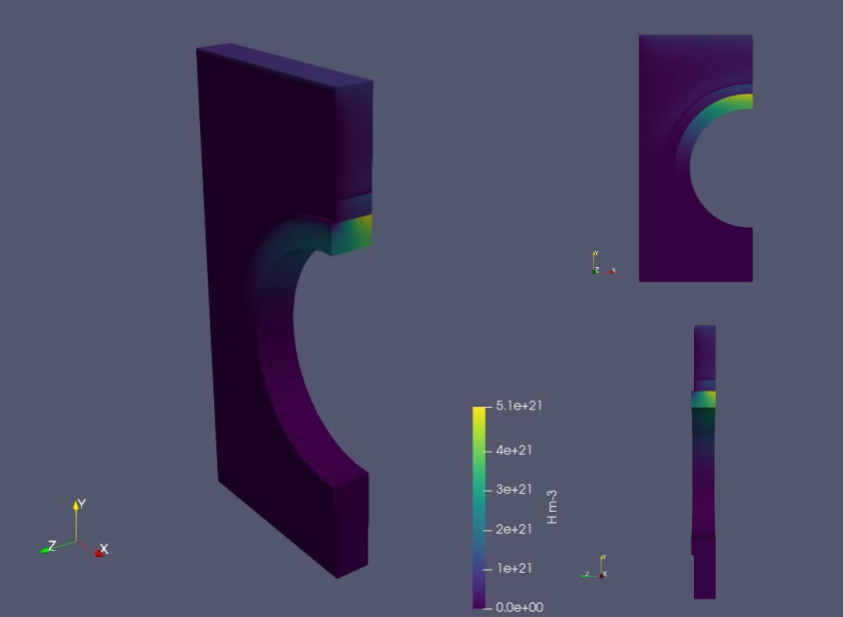
\includegraphics[width=\linewidth]{Figures/Chapter3/monoblocks/3D_monoblocks/MB 3D desorption.png}
        \caption{Instantaneous recombination on the gaps.}
    \end{subfigure}
    \begin{subfigure}{\linewidth}
        \centering
        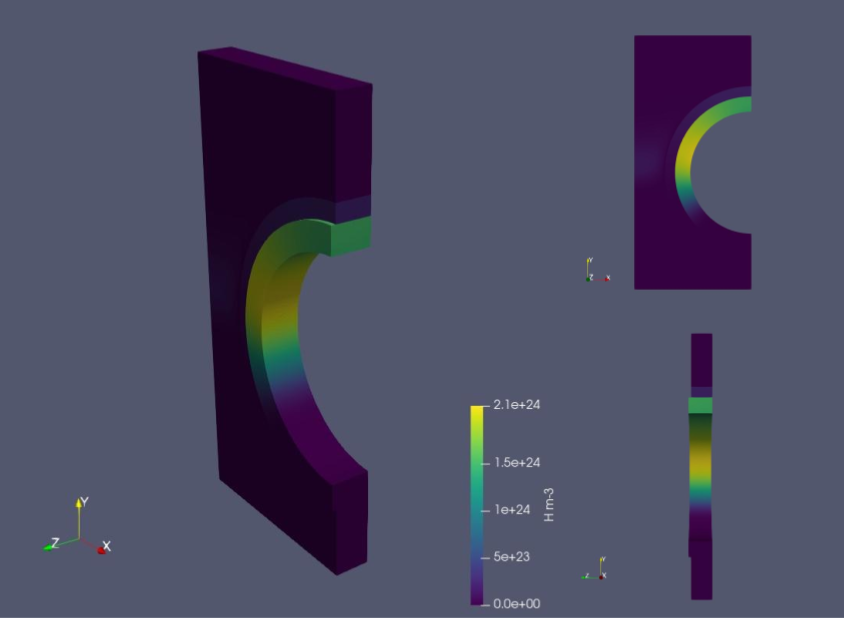
\includegraphics[width=\linewidth]{Figures/Chapter3/monoblocks/3D_monoblocks/MB 3D no desorption.png}
        \caption{No desorption on the gaps.}
    \end{subfigure}
    \caption{Retention fields of the DEMO monoblock with or without recombination on the gaps showing the isometric view (left), a central slice (top right) and a central clip showing the cooling pipe (bottom right).}
\end{figure}

\begin{figure}
    \centering
    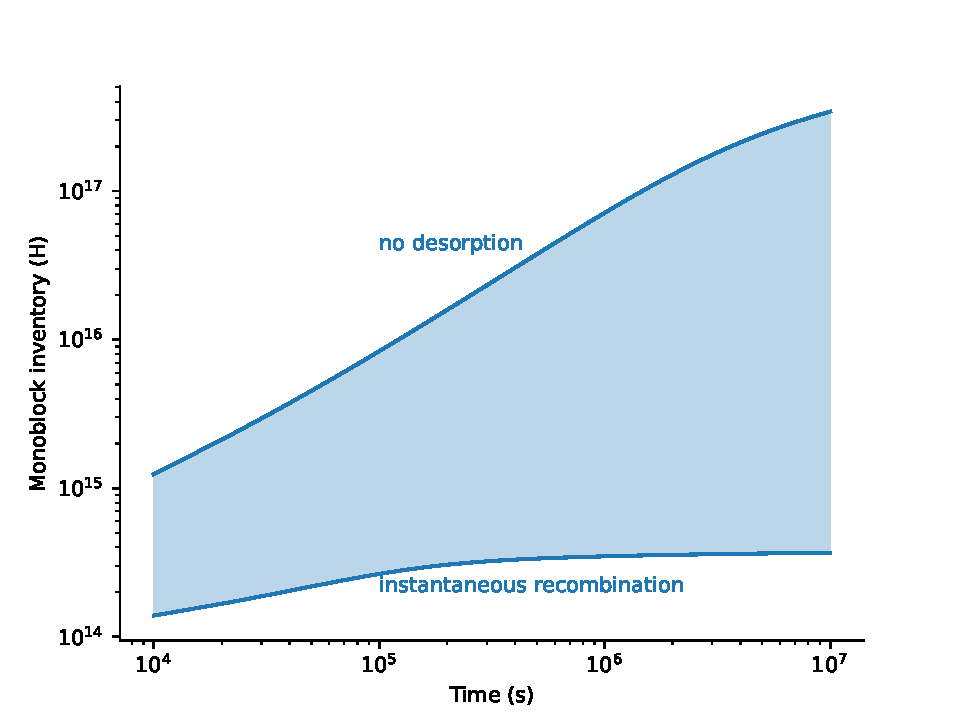
\includegraphics[width=\linewidth]{Figures/Chapter3/monoblocks/3D_monoblocks/inventory.pdf}
    \caption{Temporal evolution of the monoblock inventory.}
\end{figure}


\begin{figure}
    \centering
    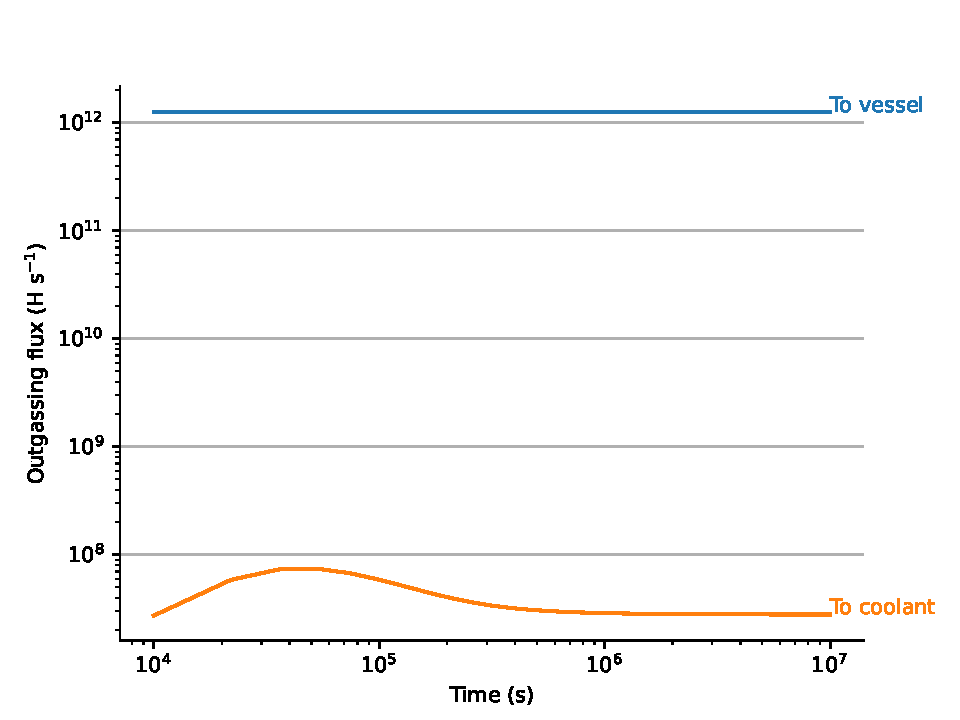
\includegraphics[width=\linewidth]{Figures/Chapter3/monoblocks/3D_monoblocks/fluxes.pdf}
    \caption{Temporal evolution of outgassing fluxes.}
\end{figure}

\subsection{Influence of the monoblock thickness}

\begin{figure}
    \centering
    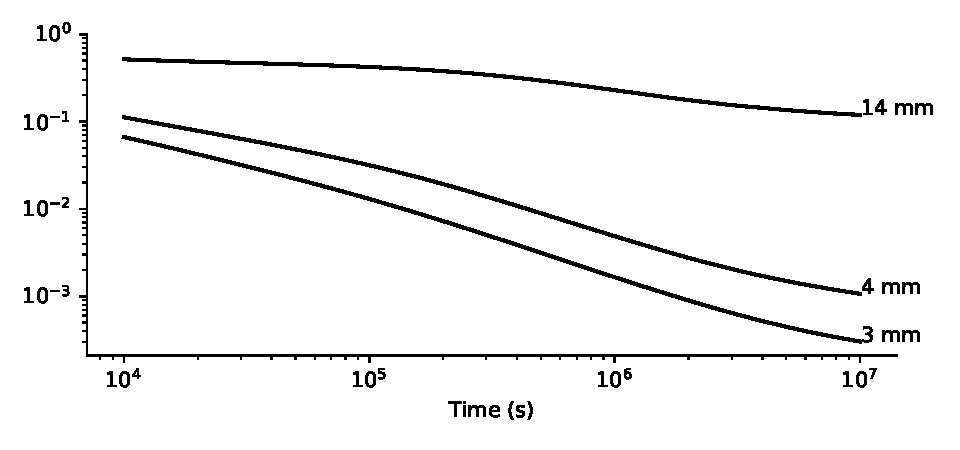
\includegraphics[width=\linewidth]{Figures/Chapter3/monoblocks/3D_monoblocks/influence_of_thickness.pdf}
    \caption{Temporal evolution of the ratio $\mathrm{inv}_\mathrm{desorption} / \mathrm{inv}_\mathrm{no desorption}$ for several thicknesses.}
\end{figure}

\subsection{Summary}